
\documentclass[a4paper]{article}\usepackage[]{graphicx}\usepackage[]{color}
%% maxwidth is the original width if it is less than linewidth
%% otherwise use linewidth (to make sure the graphics do not exceed the margin)
\makeatletter
\def\maxwidth{ %
  \ifdim\Gin@nat@width>\linewidth
    \linewidth
  \else
    \Gin@nat@width
  \fi
}
\makeatother

\definecolor{fgcolor}{rgb}{0.345, 0.345, 0.345}
\newcommand{\hlnum}[1]{\textcolor[rgb]{0.686,0.059,0.569}{#1}}%
\newcommand{\hlstr}[1]{\textcolor[rgb]{0.192,0.494,0.8}{#1}}%
\newcommand{\hlcom}[1]{\textcolor[rgb]{0.678,0.584,0.686}{\textit{#1}}}%
\newcommand{\hlopt}[1]{\textcolor[rgb]{0,0,0}{#1}}%
\newcommand{\hlstd}[1]{\textcolor[rgb]{0.345,0.345,0.345}{#1}}%
\newcommand{\hlkwa}[1]{\textcolor[rgb]{0.161,0.373,0.58}{\textbf{#1}}}%
\newcommand{\hlkwb}[1]{\textcolor[rgb]{0.69,0.353,0.396}{#1}}%
\newcommand{\hlkwc}[1]{\textcolor[rgb]{0.333,0.667,0.333}{#1}}%
\newcommand{\hlkwd}[1]{\textcolor[rgb]{0.737,0.353,0.396}{\textbf{#1}}}%

\usepackage{framed}
\makeatletter
\newenvironment{kframe}{%
 \def\at@end@of@kframe{}%
 \ifinner\ifhmode%
  \def\at@end@of@kframe{\end{minipage}}%
  \begin{minipage}{\columnwidth}%
 \fi\fi%
 \def\FrameCommand##1{\hskip\@totalleftmargin \hskip-\fboxsep
 \colorbox{shadecolor}{##1}\hskip-\fboxsep
     % There is no \\@totalrightmargin, so:
     \hskip-\linewidth \hskip-\@totalleftmargin \hskip\columnwidth}%
 \MakeFramed {\advance\hsize-\width
   \@totalleftmargin\z@ \linewidth\hsize
   \@setminipage}}%
 {\par\unskip\endMakeFramed%
 \at@end@of@kframe}
\makeatother

\definecolor{shadecolor}{rgb}{.97, .97, .97}
\definecolor{messagecolor}{rgb}{0, 0, 0}
\definecolor{warningcolor}{rgb}{1, 0, 1}
\definecolor{errorcolor}{rgb}{1, 0, 0}
\newenvironment{knitrout}{}{} % an empty environment to be redefined in TeX

\usepackage{alltt}

%--- Load packages. 
\usepackage{amssymb}
\usepackage{amsmath}
\usepackage{framed}
\usepackage{textcomp}

% avoid ugly indentation of paragraphs
\usepackage{parskip}
\usepackage{graphicx}

% open sans font
\usepackage[default,osfigures,scale=0.95]{opensans}

% subfolder with the figures (within manuscript/)
\graphicspath{ {./figures/} }

% for author affiliations
\usepackage{authblk}

%allows inline citations
\usepackage[round]{natbib}
\bibliographystyle{plainnat}

% for degree symbol
\usepackage{gensymb}

% for line numbers
\usepackage{lineno}

% margin size
\usepackage{geometry}
\geometry{verbose,tmargin=3cm,bmargin=3cm,lmargin=3cm,rmargin=3cm}

% for bibtex
% \usepackage{authordate1-4}
% \bibliographystyle{authordate1}

%allows subscripts in text mode
\usepackage{fixltx2e}

%allows rotation of table??
\usepackage{rotating} 

%allows alignment of caption to the left
\usepackage{caption} 
\captionsetup[table]{singlelinecheck=false}

%allows not italic greek letters
\usepackage{textgreek}
\IfFileExists{upquote.sty}{\usepackage{upquote}}{}
\begin{document}

\linenumbers

\title{Effects of below-ground space limitation on performance of Eucalyptus seedlings:  Does photosynthesis really control growth?}

\author[1,3]{Courtney E. Campany}
\author[2]{Belinda E. Medlyn}
\author[1]{Remko A. Duursma}

\affil[1]{Hawkesbury Institute for the Environment, University of Western Sydney, Richmond, NSW 2753, Australia}
\affil[2]{Department of Biological Sciences, Macquarie University, North Ryde, NSW 2109, Australia}
\affil[3]{Corresponding author (c.campany@uws.edu.au)}

\renewcommand\Authands{ and }
\maketitle

%--------------------------------------------------------------------------------------------%




%--------------------------------------------------------------------------------------------%

\section*{Abstract}

Interpreting limitations to plant growth requires understanding of the balance between carbon (\textit{C}) source and sink activity in order to assess \textit{C} allocation and biomass partitioning. This study used manipulations of soil volume to test how growth is coupled to physiology, allocation, and sink activity in \textit{Eucalyptus tereticornis} seedlings. We grew seedlings in a large range of container sizes and planted containers flush to the soil alongside naturally sown seedlings (free). Reduced soil volume was expected to induce rapid negative effects on growth and physiology compared to free seedlings. It was hypothesized that soil volume effect would be largest in the smallest containers, resulting in physical constraints to growth independently of photosynthesis (\textit{A}). Photosynthesis would then become sink-limited, resulting in the build-up of leaf nonstructural carbohydrates eventually leading to photosynthetic down regulation. We observed a negative container effect on aboveground growth soon after the experiment started. Although growth was consistently different across soil volumes mass, partitioning to leaves, stems, roots was conserved after 120 days. Photosynthetic capacity was also significantly reduced in containers, and was related to both leaf nitrogen content and starch accumulation. We developed a seedling growth model that utilized leaf \textit{A} rates to allocate daily \textit{C} uptake towards mass growth of stems, leaves and roots. We then asked whether the observed reductions in \textit{A} explained the observed differences in seedling biomass. We found that although belowground sink limitation resulted in the down regulation of \textit{A}, these reductions could not explain observed growth responses. Thus, as photosynthesis and growth were not coordinated a pool of excess \textit{C} resulted in seedlings with soil volume restriction. This research highlights the need to further utilize mass balance approaches when evaluating plant \textit{C} allocation and confirms that \textit{A} and growth are not always directly related.

\section*{Key Words}

photosynthesis, sink regulation, growth, carbon allocation, soil volume


\section*{Introduction}

Understanding plant growth requires knowledge of the mass balance that must be achieved between \textit{C} uptake and subsequent allocation to growth, storage, and respiration. It is commonly assumed plant growth is limited by \textit{C} availability, yet it has long been demonstrated that correlations between \textit{A} and growth are weak or seldom present. \citet{korner2013growth} argues that growth instead controls \textit{A}, as it is the norm for sink activity to feedback on source activity. This is supported by evidence that growth of plants under environmental stress is not limited by the supply of photoassimilates \citep{palacio2014does}. As woody plants have highly integrated systems of competing carbohydrate sinks \citep{kozlowski1992carbohydrate}, growth should principally depend on the transport of these photoassimilates between different tissue and organ sinks. Despite a wealth of studies, however, large uncertainties still remain regarding the coordination of \textit{C} supply, via \textit{A}, and growth of woody species.

In woody species, how \textit{A} controls growth has been studied with manipulations of \textit{C} source activity. Examples included elevated CO\textsubscript{2} experiments, for example FACE (reviewed in  \citet{ainsworth2005have}, and partial defoliation experiments. Elevated CO\textsubscript{2} has been shown to increase \textit{A} rates \citep{drake1997more,ainsworth2007response} and across four FACE experiments this resulted in a conserved increase in forest production \citep{norby2005forest}. Evidence from elevated CO\textsubscript{2} experiments, however, also reveals that the growth response tends to be much smaller than the photosynthetic enhancement \citep{kirschbaum2011does}. In defoliation experiments, compensatory increases in \textit{A} are commonly shown yet are attributed to variable mechanisms, including reduction in end product inhibition \citep{iglesias2002regulation,zhou2003changes,handa2005test}, enhanced biochemical activity \citep{ovaska1993b,layne1995end}, increased stomatal conductance \citep{layne1995end}, leaf nutrient status \citep{turnbull2007increased}, and regulatory sugar signaling \citep{eyles2013whole}. However, increases in \textit{A} did not always produce increased growth due to reductions in meristem sink strength (Palacio et al. 2012), \textit{C} limitation to mycorrhizal colonization (Markkola et al. 2004), or an overall decrease in whole plant \textit{C} gain \citep{ovaska1993a}. These manipulations of \textit{C} source activity expose unresolved issues with how changes in \textit{A} do not always infer similar responses in growth.

Alternatively, tissue sink activity can restrict biomass production when limited by environmental or developmental constraints \citep{korner2003carbon}. This is because metabolic signaling networks, relaying information on \textit{C} and nitrogen (\textit{N}) status of different tissues, can down regulate photosynthetic activity \citep{paul2001sink}.  Whether this down regulation, via sink inhibition, exists in woody species has been tested through fruit removal, girdling, and low temperatures. In these studies, down regulation of \textit{A} was frequently correlated to carbohydrate accumulation resulting from reduced tissue sink strength \citep{iglesias2002regulation,hoch2002altitudinal,urban2007girdling, haouari2013fruit}. However, reductions in \textit{A} were also attributed to biochemical limitations prior to carbohydrate accumulation \citep{nebauer2011photosynthesis}, irreversible photo-oxidative damage \citep{duan2008photosynthetic}, and stomatal limitation \citep{li2005photosynthesis}. These mixed results are not surprising as we still know little about the pathways in which plants achieve balance between assimilation, storage, and growth across temporal scales \citep{smith2007coordination}. As these manipulations likely impact source as well as sink activity simultaneously, affect water transport, are very extreme, or are specific to large annual fruiting sinks, they tell us little about source-sink coordination in ‘normal’ field-grown woody species. This coordination is further confounded by the fact that under normal growing conditions, \textit{A} is not always correlated to photosynthate accumulation, as with fir needles \citep{little1973effect}. Unfortunately, there is still limited understating of the physiological roles of carbohydrates in photosynthetic regulation and the elements triggering the down-regulation process \citep{nebauer2011photosynthesis}. 

An alternative approach is to lower belowground \textit{C} sink strength in tree seedlings by manipulating rooting volume, by varying the container size. The advantage of this approach is it allows a large range of manipulations, can be easily compared to naturally planted seedlings and mimics natural conditions as seedlings compete for space or reach bedrock. Seedlings undergo many physiological and morphological changes in response to rooting volume, including biomass partitioning, \textit{A}, water relations, nutrient uptake and respiration \citep[and references therein]{nesmith1998effect}. The rooting volume available to plants can decrease \textit{C} sink strength by reducing root growth. Container size studies frequently have photosynthetic down-regulation, likely as a result of sink limitation \citep{arp1991effects, mcconnaughay1991physical, gunderson1994photosynthetic, sage1994acclimation, maina2002intra, ronchi2006growth}. A meta-analysis by \citet{poorter2012pot} concluded that \textit{A} is the process likely to be the strongest affected by pot size and may best explain the observed effect on biomass seen in the large number of studies where containers are used. This conclusion arises because plants grown in small containers are shown to accumulate leaf starch while having lower \textit{C} exchange and assimilate export rates \citep{robbins1988effect}. However, evidence in support for a trade-off between \textit{C} storage and growth in trees is, to date, inconclusive \citep{palacio2014does}. Based on these previous studies, using container size as a sink-strength manipulation can be used to empirically test how growth and \textit{A} are coordinated.

Another barrier in understanding the coordination between \textit{A} and growth is a lack of knowledge regarding the allocation of \textit{C} in woody species.  Understanding the fate of assimilated \textit{C} is crucial when source or sink manipulations do not directly lead to equivalent changes in growth. As programmed plasticity in \textit{C} allocation naturally occur as plants growth and develop, this must be accounted for when evaluating induced variation in growth \citep{wright2002interpreting}. Thus, when \textit{C} allocation is altered by a treatment, it should be shown whether these allocation patterns differ from common sized untreated plants \citep{reich2002root, poorter2012biomass}. Only then can we test if functional balance preservation or optimal foraging occurs from changes in \textit{C} uptake. For example, seedlings in containers may shift allocation to leaves if root restriction occurs or alter fine root morphology to increase nutrient uptake. In woody species, shifts in allometric relationships of leaves, stems and roots can reveal if growth is ontogenetically constrained or actively adjusted when \textit{A} is affected. This then allows additional pools of \textit{C}, such as root exudation or changes in tissue respiration, to be accounted for and evaluated.

This study utilizes a novel field design to investigate the coordination between growth and \textit{A} in \textit{Eucalyptus tereticornis} Sm.~seedlings, by manipulating container size and thus rooting volume. Seedlings were maintained under well watered conditions in order to evaluate only the effect of restricted soil volume and the limited nutrient resource pool. We used freely-rooted seedlings as a control for the container size treatments.  Empirical results were combined with a simple plant growth model to simulate seedling growth with a \textit{C} mass balance approach, which was then compared to observed harvested seedling mass.  The model used whole-plant \textit{C} gain, scaled from instantaneous rates of leaf \textit{A}, to quantify seedling production over 120 days. 

1). The manipulations of container size were hypothesized to induce a belowground sink limitation in these seedlings      which was expected to be largest in the smallest containers, resulting in physical constraints to growth independently of \textit{A}.

2). Reducing soil volume was expected to induce rapid negative effects on growth and physiology compared to free seedlings (‘container effect’), with accumulation of leaf nonstructural carbohydrates triggering photosynthetic down regulation through time as a function of available soil volume.

3). Last, the growth model was expected to find agreement between simulated and observed seedling mass, through direct correlation of the effects of soil volume on rates of leaf \textit{A}.

\section*{Methods}

\subsection*{\textit{Experimental Design}}

This experiment was located on the Hawkesbury Forest Experiment site in Richmond, NSW, Australia. Plots were located in open cover with a site history that consists of a paddock that was converted from native pasture grasses. Top soils at this site, used for the study, are an alluvial formation of low-fertility sandy loam soils (380 and 108~mg~kg\textsuperscript{-1} total \textit{N} and phosphorus respectively) with low organic matter (0.7~\%) and low water holding capacity. At this site a soil hard layer exists at $\sim$1.0~m with a transition to heavy clay soils. The climate for the region is classified as sub-humid temperate. 

\textit{Eucalyptus tereticornis} seedlings, 20~weeks old and approximately 40~cm tall in tube stock, were chosen from a single local Cumberland plain cohort. Previous experiments have confirmed that species with tap roots (similar to \textit{E. tereticornis}) use the center of the container as the medium for thick roots leaving the periphery of the soil as the most active sites for fine root proliferation \citep{biran1980a,biran1980b}. This is generally hypothesized to be a different response than seedlings with no taproot. By using a species with tap root growth and manipulations of container length rather than width, it is believed that a more realistic test of inhibition of growth through constrained soil volume would be achieved. Six seedlings were harvested before planting to measure initial leaf area and dry mass of leaves, stems and roots.

Six container volumes were used ranging from 5~l to 35~l, with a 22.5~cm diameter, and lengths ranging from 15 to 100~cm. Containers were constructed of PVC pipe and were filled with local top soil (described above). Soil in each container was packed to achieve a target soil bulk density of 1.7~g~m\textsuperscript{-3}. A Imidacloprid (BAYER CropScience) insecticide tablet was planted 5 cm below the roots of each seedling. Containers were planted flush with the soil surface inside metal sleeves, designed to minimize excess air space between the container and outside soil while also allowing for container removal. This allowed for soil temperatures in containers to reflect conditions of naturally sown (free) seedlings. Each experimental block (n=7) contained a complete replicate set of container volumes as well as one free seedling, with 1 m\textsuperscript{2} spacing. For each free seedling, a 1~m\textsuperscript{2} subplot was excavated to 0.5~m and replaced with the same soil used in each container. A border of root exclusion material was buried 0.25~m deep and extended 0.25~m above the ground surface around each subplot to exclude local vegetation.

Plants were watered weekly or when needed, accounting for natural precipitation, to maintain soil moisture at field capacity (13-15~\%). Drain systems were built into each pot to prevent pooling of water in containers before root expansion, from reduced root uptake, or from large rainfall events. These conditions could lead to an anaerobic environment around the root that could hinder the uptake of water through reduced root conductance \citep{poorter2009causes}, an undesired experimental artifact. A collection compartment in the bottom of containers, containing gravel covered by root exclusion mesh, was used to collect excess water for 20, 25, and 35~l containers. Plastic tubing (6~mm diameter) was inset into the gravel layer and extended through the top of the container. A lysimeter pump was then used to suction excess water, through the tubing, as needed. As small containers (5, 10, and 15~l) have a larger irradiation effect a simple bottom plug was used to drain excess water from the gravel compartment.  

\subsection*{\textit{Growth and morphology metrics}}
Seedlings were planted on January 21\textsuperscript{st} 2013 and stem height, diameter at 15~cm and leaf count were measured weekly thereafter. Once the growth rate of individual plants had significantly declined a full biomass harvest was completed (May 21\textsuperscript{st} 2013). Dry mass of leaves, stems, roots and cumulative leaf area (LI-3100C Area Meter; LI-COR, Lincoln, NE, USA) was measured for each seedling. Mean individual leaf area for each harvested seedling was calculated by dividing cumulative leaf area by total leaf count of only fully expanded leaves. This value was then used to interpolate cumulative leaf area through time with weekly leaf counts. Root mass was collected by passing soil from each container through a 1~mm sieve, washing, separating into fine and coarse roots (\textless2~mm and \textgreater2~mm diameter, respectively) and then drying to a constant mass. Roots from the free seedlings were collected by excavating each 1~m\textsuperscript{2} subplot to 0.5~m depth.  25~g fresh weight subsamples of washed fine roots were analyzed, using WhinoRhizo software (Regent Instruments Inc.), for specific root length (SRL, cm~m\textsuperscript{-1}).

\subsection*{\textit{Photosynthetic parameters}}
Leaf gas exchange measurements were performed bi-weekly at saturating light (\textit{A}\textsubscript{sat}) and saturating light and [CO\textsubscript{2}] (\textit{A}\textsubscript{max}) on new fully expanded leaves. Measurements were initiated only after sufficient new leaf growth occurred (March 17\textsuperscript{th}, 2013), approximately 6 weeks following planting, and continued until the biomass harvest. Leaf level gas exchange was measured with a standard leaf chamber equipped with blue-red light emitting diodes using a portable gas exchange system (LI-6400, LI-COR, Lincoln, NE, USA). \textit{A}\textsubscript{sat} measurements were made at PPFD of 1800~{\textmugreek}mol~m\textsuperscript{-1}~s\textsuperscript{-1} and [CO\textsubscript{2}] of 400~{\textmugreek}l~l\textsuperscript{-1} and \textit{A}\textsubscript{max} with [CO\textsubscript{2}] of 1600~{\textmugreek}l~l\textsuperscript{-1} and PPFD of 1800~{\textmugreek}mol~photons~m\textsuperscript{-1}~s\textsuperscript{-1}. This choice of light level to achieve light saturation is consistent with other studies on \textit{Eucalyptus} species \citep{kallarackal1997ecophysiological,pinkard1998photosynthetic,crous2013photosynthesis,drake2014capacity}. These measurements were conducted during midday (10:00-14:00~h) with leaf temperature maintained at 25$\degree$C. After leaves acclimated to the chamber environment, net CO\textsubscript{2} assimilation rate and stomatal conductance (\textit{g}\textsubscript{s}) were logged 5 times for both \textit{A}\textsubscript{sat} and \textit{A}\textsubscript{max}. Photosynthetic CO\textsubscript{2} response (AC\textsubscript{i}) curves were also developed at 25$\degree$C on a random subset of each container size (n=3) after new leaves were first produced and immediately prior to the final harvest (May 23\textsuperscript{rd} 2013). Each AC\textsubscript{i} curve began at the reference [CO\textsubscript{2}] of 400~{\textmugreek}l~l\textsuperscript{-1} and then consisted of 12 additional steps from [CO\textsubscript{2}] of 50 to 1800~{\textmugreek}l~l\textsuperscript{-1}at 25$\degree$C at saturating light (above). From these curves the photosynthetic parameters, \textit{J}\textsubscript{max} and \textit{Vc}\textsubscript{max}, were quantified using the biochemical model of \citet{farquhar1980biochemical}. Leaf dark respiration rates (\textit{R}\textsubscript{d}) was measured on each seedling during the same dates as AC\textsubscript{i} curves using detached leaves inside a conifer chamber attached to the Licor 6400 at least 1 hour after sundown.   Measurements were taken at a reference [CO\textsubscript{2}] of 400~{\textmugreek}l~l\textsuperscript{-1} while leaf temperature was maintained at current ambient conditions. Reported values of \textit{R}\textsubscript{d}) reported are predicted rates at 25$\degree$C using a Q10 value (1.86) developed on these seedlings in a separate experiment. Specific leaf area (SLA, m\textsuperscript{2}~kg\textsuperscript{-1}) was calculated by measuring leaf area and dry mass for all individual leaves sampled during gas exchange campaigns.

\subsection*{\textit{Leaf water potential}}
Predawn ($\Psi\textsubscript{pd}$) and midday ($\Psi\textsubscript{l}$) leaf water potentials were measured for each seedling using a PMS 1505D pressure chamber (PMS Instruments, Albany, OR, USA) on fully expanded leaves during the same time period as AC\textsubscript{i} and \textit{R}\textsubscript{d}. Leaves were detached and immediately stored inside foil covered bags before water potential measurements were performed. $\Psi\textsubscript{pd}$ was measured before sunrise and $\Psi\textsubscript{l}$ at midday 13:00-14:30~h. These measurements were used as a measure of static water stress on the seedlings \citep{sellin1999does}, and to ensure that the bulk soil water availability was high enough for plants as they became larger and roots filled the soil volume. 

\subsection*{\textit{Leaf, root and soil chemistry}}
Leaves used in each gas exchange measurements and subsamples of harvested roots were dried to a constant mass and milled for analysis of \textit{N} content,{\textdelta}\textsuperscript{13}C, and total non-structural carbohydrates (TNC). Pre-planting soil samples (n=6) and subsamples of soil from each container following harvest were sieved to remove organic material, air dried and milled for analysis. \textit{N} concentrations of leaf and soil samples were determined using a Carlo Erba CE1110 elemental analyzer with thermal conductivity and mass spectromic detection (of \textit{N}\textsubscript{2} and CO\textsubscript{2}).  The percentage of \textit{N} in the sample was calculated by comparison with known standards. Leaf {\textdelta}\textsuperscript{13}C was analyzed  with an Delta V Advantage coupled to a Flash HT and Conflo IV isotope ratio mass spectrometer. Leaf samples were flash combusted at 1000$\degree$C to convert to to CO\textsubscript{2}, feed to the mass spectrometer and isotopic signatures are reported relative to the VPDP scale. Leaf TNC concentration was analyzed using a total starch assay kit (Megazyme International 303 Ireland Ltd., Wicklow, Ireland) and includes the starch (mg~g\textsuperscript{-1}) and soluble sugar (mg~g\textsuperscript{-1}) concentrations. Starch was quantified using a thermostable $\alpha$-amylase and amyloglucosidase assay \citep{McCleary_starch} and soluble sugars were determined following the anthrone method \citep{ebell1969variation}. Complete methods of the TNC assay are described in \citep{mitchell2013drought}.

\subsection*{\textit{Seedling growth model}}
We developed a simple seedling growth model that utilized leaf \textit{A} rates to allocate daily \textit{C} assimilate towards biomass production of stems, leaves, fine roots and coarse roots. The model begins with mean initial tissue component biomass (leaf\textsubscript{i}, stem\textsubscript{i} and root\textsubscript{i}) and a starting leaf area (LA\textsubscript{i}) measured prior to planting. The initial biomass of roots was divided evenly between fine and coarse roots. The daily net biomass production of seedlings (P\textsubscript{i}) is then given by
\begin{equation} P\textsubscript{i}=L~C\textsubscript{day,i}~\epsilon\textsubscript{c}\textsuperscript{-1}-R
\label{eq:prod}
\end{equation}
where L is standing cumulative leaf area, C\textsubscript{day,i} is the predicted mean daily carbon assimilation, \textepsilon\textsubscript{c} is a biomass conversion efficiency parameter and R is the total respiration of all tissue components. Total respiration was calculated as 
\begin{equation} R=\Sigma(R\textsubscript{c}~M\textsubscript{c})
\label{eq:resp}
\end{equation}
where R\textsubscript{c} is tissue respiration of fine roots, coarse roots or stems on a mass basis and M\textsubscript{c} is the standing biomass of each component. R\textsubscript{leaf} is represented in the calculation of C\textsubscript{day}. The change in individual component biomass, here solved on a daily time step, is given by
\begin{equation} \frac{dM\textsubscript{c}}{dt}=A\textsubscript{c}~P\textsubscript{i}-(\Lambda\textsubscript{c}~M\textsubscript{c})
\label{eq:mass}
\end{equation}
where A\textsubscript{c} is the component specific biomass partitioning  to whole plant biomass (\%) and $\Lambda\textsubscript{c}$ is component specific turnover rate. Due to the duration of the experiment $\Lambda\textsubscript{stem}$ was assumed to equal 0.  Total seedling biomass, per time step, was then equal to the sum of all biomass components; leaves, stems, fine roots and coarse roots. 

\textit{C}\textsubscript{day} was predicted by fitting a coupled photosynthesis - stomatal conductance model \citep{farquhar1980biochemical,medlyn2011reconciling} in the 'plantecophys' package in R \citep{Duursma2014} to the mean photosynthetic parameters (R\textsubscript{d}, J\textsubscript{max}, V\textsubscript{cmax}, and g\textsubscript{1}) for each treatment and meteorological data from an onsite weather station.  Examples of the photosynthesis model are described in \citet{medlyn2002temperature} and the approach of the coupled leaf gas exchange model are described in \citet{duursma2014peaked}. The g\textsubscript{1} parameter was generated by fitting observed \textit{g}\textsubscript{s} values into the optimal stomatal conductance model from \citep{medlyn2012reconciling}. Combined with the meteorological parameters; PPFD, air temperature, and relative humidity, at 15~m intervals, leaf \textit{A} rates ({\textmugreek}mol~CO\textsubscript{2}~m\textsuperscript{-2}~s\textsuperscript{-1}) were predicted for each soil volume treatment. Rates were assumed to be representative of the entire 15~min meteorological interval. \textit{C}\textsubscript{day} was calculated by converting predicted rates to mass \textit{C} gain over 15~min (g~m\textsuperscript{-2}) and then summed for 24~h. This resulted in 120 unique values of \textit{C}\textsubscript{day} for each soil volume treatment, one value for each day of the experiment. Thus, each daily time step for model runs included a value of \textit{C}\textsubscript{day} that represented both treatment specific photosynthetic parameters and meteorological constraints across the duration of the experiment. All default parameters used in model simulations are reported in Table.~\ref{table:Table3}.

We then utilized this model to test the hypothesis that the effects of belowground sink limitation on rates of leaf \textit{A} where sufficient to accurately predict overall seedling production after 120 days. Each model was run with a sequence of \textit{C}\textsubscript{day}  values (n=101) covering the entire range of predicted values of all soil volume treatments and the free seedling control. First, the model was simulated using only changes in \textit{A} rates across treatments, via \textit{C}\textsubscript{day}, combined with mean values of mass partitioning and either published or local data of stem and root respiration rates (M\textsubscript{0}). Next, the model was fit with with treatment specific mass partitioning from the final harvest (M\textsubscript{1}) in order to determine how ontogenetic differences in seedling allometry improved biomass predictions. Finally, model sensitivity to 3 different \textit{C} allocation scenarios, including changes to leaf \textit{C} allocation, root respiration rates, and fine root \textit{C} allocation (M\textsubscript{2,3,4} respectively), was tested to investigate possible sources of missing \textit{C} from initial model simulations. This was accomplished by testing the sensitivity of the model to adjustments of \textit{C} allocation to leaves, fine roots or root respiration rates by $\pm$50~\% of default values. For all cases, biomass production was compared between model output and harvested seedlings. 

\subsection*{\textit{Data Analysis}}
Differences in experimental parameters with soil volume were analysed by one-way analysis of variance (ANOVA) in R with individual containers as random effects and soil volume as a categorical fixed effect. Tukey’s post-hoc tests were performed in conjunction with ANOVA to determine which specific paired comparisons among soil volume treatments were different. Mixed model ANOVAs of \textit{A}\textsubscript{max} and leaf chemistry were performed using the 'nlme' package \citep{nlme} in R and \textit{r}\textsuperscript{2} values of mixed models were computed as in \citet{nakagawa2013general}. Tests of allometric relationships between biomass components were implemented using major axis regression in the 'smatr' package in R \citep{warton2012smatr}. Results were considered significant at P$\leq$0.05.

\section*{Results}

\subsection*{\textit{Growth and morphology metrics}}
In this open field study, colder temperatures and reductions in cumulative PPFD per day (Fig.~\ref{fig:figure1}) most likely lead to the reduced growth in the free seedlings in the final weeks of the experiment (Fig.~\ref{fig:figure2}).  Combined with severe growth reductions in the smallest container volumes the experiment was chosen to be harvested after 120~days. Over this duration height, diameter, and leaf area diverged between container volumes (Fig.~\ref{fig:figure2}).  First, seedling leaf area significantly diverged between soil volumes (\textit{P}\textless0.026) during the 5\textsuperscript{th} week of the experiment. Following this period both height (8\textsuperscript{th} week) and then diameter (9\textsuperscript{th} week) significantly deviated across soil volumes (\textit{P}\textless0.002 \& 0.001, respectively).  Negative growth effects then manifested as severely reduced height gain and declining leaf area through time with small soil volumes across the final two months of the experiment. Seedlings maintained diameter growth throughout the experiment, although marginal with smaller soil volumes in the final month. Final seedling height significantly increased with increasing soil volume (\textit{P}\textless0.001).  Increases in both final stem diameter (\textit{P}\textless0.001) and cumulative leaf area (both \textit{P}\textless0.001) were found with increasing soil volume and these differences were driven mainly by the largest container and the free seedling.

Harvested total seedling biomass at harvest was significantly different across container volumes (\textit{P}\textless0.001) and with free seedlings (\textit{P}\textless0.001, Table.~\ref{table:Table1}). We analyzed the relationship between biomass growth with each fold increase in soil volume and found an increase of 34~\% with a doubling of pot size, consistent with the meta-analysis of \citet{poorter2012pot}. Additionally, plant biomass was highly correlated with total leaf area across all treatments (\textit{r}\textsuperscript{2} = .97, \textit{P}\textless0.001). Differences in biomass partitioning to leaves, stems, and roots were not different across soil volumes when variation in seedling biomass within treatments was factored in the analysis. Across all treatments, the final harvested root:shoot was conserved in these seedlings, with a slightly higher shoot than root mass on average ($\overline{x}$=0.904).

SRL of harvested fine roots was not different across soil volumes (Table.~\ref{table:Table1}). Over the duration of the experiment SLA was higher in free seedlings but was not different across containers sizes (Table.~\ref{table:Table1}, \textit{P}\textless0.001) and this pattern was evident in the first gas exchange measurement campaign (\textit{P}\textless0.001).

\subsection*{\textit{Leaf and root chemistry}}
Leaf \textit{N}~\% was significantly higher in free seedlings and the largest container volume at the onset of gas exchange measurements (6th week, \textit{P}\textless0.001).  Over the remaining duration of the experiment the smallest container volume had a significant reduction in leaf \textit{N}~\% compared to other soil volumes, while free seedlings maintained a greater leaf \textit{N}~\% (Table.~\ref{table:Table1}, \textit{P}\textless0.001).  Additionally, mean leaf starch content in the smallest container was double that of free seedlings (\textit{P}=0.042), while leaf soluble sugars did not differ across treatments throughout the experiment (Table.~\ref{table:Table1}).  Differences in leaf starch between the free seedling and the smallest container were also evident during the first gas exchange campaign (\textit{P}=0.0013). 

\subsection*{\textit{Gas exchange and photosynthetic parameters}}
\textit{A}\textsubscript{sat} (Fig.~\ref{fig:figure3}) and \textit{A}\textsubscript{max} (Table.~\ref{table:Table2}) were both significantly higher in the largest container volume and the free seedling at the first measurement campaign (both \textit{P}\textless0.001). Across measurement campaigns \textit{A}\textsubscript{sat} was consistently higher in free seedlings than in containers (Figure 3, \textit{P}\textless0.001). The interaction between photosynthetic capacity, leaf starch, and leaf \textit{N} on a mass basis was marginally significant (\textit{P}=0.0584) but \textit{A}\textsubscript{max} was highly correlated to both leaf \textit{N} content and leaf starch (both \textit{P}\textless0.001). Across all measurement campaign \textit{A}\textsubscript{max} was higher when foliar \textit{N} was also higher, usually associated with low levels of leaf starch (Fig.~\ref{fig:figure3}a). \textit{A}\textsubscript{max} was also lower when leaf starch was high as higher leaf \textit{N} often did not coincide with high leaf starch (Fig.~\ref{fig:figure3}b)

The photosynthetic parameters~\textit{J}\textsubscript{max} and~\textit{Vc}\textsubscript{max} were not different across measurement campaigns, therefore the parameter means per treatment are reported here (Table.~\ref{table:Table2}).  Overall, both \textit{J}\textsubscript{max} and \textit{Vc}\textsubscript{max} were significantly higher in free seedlings with little variation between soil volume treatments(\textit{P}=0.0012 \& 0.0021, respectively). Leaf dark respiration rates were not significantly different across soil volumes (Table.~\ref{table:Table2}). The \textit{g}\textsubscript{1} parameter, generated for each seedling from the \citet{medlyn2012reconciling} optimal stomatal conductance model, was not different across soil volumes (Table.~\ref{table:Table2}). Predicted values of \textit{g}\textsubscript{s}, using the \textit{g}\textsubscript{1} parameter, where highly correlated with observed values (\textit{r}\textsuperscript{2}= .74, \textit{P}\textless0.001, data not shown).

Neither $\Psi\textsubscript{pd}$ nor $\Psi\textsubscript{l}$ were different across treatments, with mean values of -0.27 and -1.2~mPa across all seedlings, respectively. Although \textit{g}\textsubscript{s} in free seedlings was generally higher than those in containers (Table.~\ref{table:Table2}, \textit{P}=0.0023), the mean rates for all seedlings were high at 0.37~mol~H\textsubscript{2}0~m\textsubscript{-2}~s\textsubscript{-1} and did not decline significantly across the experiment duration. Additionally, leaf {\textdelta}\textsuperscript{13}C at final harvest was not different across treatments (Table.~\ref{table:Table1}). Combined these indices provide strong evidence that water stress was not apparent on these well-watered seedlings throughout the experiment. Soil \textit{N}~\% at harvest was not different across soil volumes ($\bar{x}$=04.5~\%) and decreased approximately 3~\% across all containers over the experiment duration. This indicates that nutrient leaching from free seedlings or from draining of containers following natural rainfall events did not differ between treatments. 

\subsection*{\textit{Modelling seedling biomass}}
Model M\textsubscript{0}, testing only treatment specific photosynthesis rates, was found to overestimate seedling production when compared to harvested seedling biomass. When both \textit{C}\textsubscript{day} and biomass of modeled and harvested seedlings were scaled to the control treatment this overestimation was greater for seedlings with soil volume restriction (Fig.~\ref{fig:figure6}a). Model M\textsubscript{1}, using treatment specific leaf, stem and root biomass partitioning, also overestimated seedling production for all soil volume treatments (Fig.~\ref{fig:figure6}b). With both  M\textsubscript{0} and  M\textsubscript{1} this overestimation resulted in a unexplained pool of missing carbon in seedlings that was not attributed to biomass growth. Models M\textsubscript{2,3,4} were then utilized to investigate how different \textit{C} allocation scenarios, not explicitly tested within the framework of this experiment, might account for these pools of unexplained carbon. Both decreases in fine root C allocation and increases in leaf C allocation slightly improved biomass estimates but neither were sufficient to accurately predict the observed biomass response  (Fig.~\ref{fig:figureSI1}a,c). Altering respiration rates of fine and coarse roots did not have a noticeable deviation from the original model (Fig.~\ref{fig:figureSI1}b).

\section*{Discussion}


%--------------------------------------------------------------------------------------------%
\section*{Tables}
% Load xtable for printing tables.



%seedling data table
% latex table generated in R 3.1.2 by xtable 1.7-4 package
% Mon May 18 09:55:34 2015
\begin{sidewaystable}[ht]
\centering
\caption{Responses of plant and leaf characterisitics of \textit{Eucalyptus tereticornis} seedlings to soil volume treatments. Each value reflects the mean(standard error) for each treatment. Seedling mass, SRL, root nitrogen and leaf \textdelta\textsuperscript{13}C values are from final harvest. Values of leaf starch, sugars, nitrogen and SLA represent overall means across measurement campaigns (n=6). Different letters represent significant differences between treatments. The container effect P value represents the overall difference between seedlings with soil volume restriction and the control seedlings.} 
\label{table:Table1}
\begin{tabular}{lllllllll}
  \hline
Volume (L) & Seedling~mass~(g) & SLA\textsubscript{TNC-free}~(m\textsuperscript{2}~kg\textsuperscript{-1}) & Leaf~Starch~(\%) & Leaf~Sugars~(\%) & Leaf~Nitrogen~(\%) & Root~Nitrogen~(\%) & SRL~(cm~m\textsuperscript{-1}) & {Leaf~\textdelta}\textsuperscript{13}C~(\text{\textperthousand}) \\ 
  \hline
5 & 14.8 (1.82) a & 11.8 (0.32) a & 12.7 (0.97) b & 6.4 (0.28) a & 1.1 (0.02) a & 0.78 (0.04) ab & 39.1 (5.47) a & -30.1 (0.26) a \\ 
  10 & 20.0 (2.38) ab & 11.7 (0.31) a & 9.4 (0.75) ab & 6.7 (0.25) a & 1.3 (0.04) ab & 0.75 (0.02) a & 34.2 (5.83) a & -30.2 (0.25) a \\ 
  15 & 25.4 (2.49) ab & 12.7 (0.48) a & 7.3 (0.73) a & 7.2 (0.28) a & 1.4 (0.06) ab & 0.71 (0.02) a & 37.6 (4.63) a & -30.3 (0.36) a \\ 
  20 & 23.4 (1.63) ab & 11.8 (0.37) a & 9.5 (0.88) ab & 6.6 (0.26) a & 1.4 (0.05) ab & 0.76 (0.04) a & 45.3 (5.50) a & -29.7 (0.28) a \\ 
  25 & 30.4 (5.49) ab & 12.4 (0.40) a & 9.8 (0.71) ab & 6.9 (0.24) a & 1.3 (0.06) ab & 0.74 (0.02) a & 47.0 (7.10) a & -29.7 (0.25) a \\ 
  35 & 52.2 (9.55) b & 13.5 (0.46) ab & 9.8 (0.65) ab & 6.8 (0.22) a & 1.5 (0.08) b & 0.77 (0.03) ab & 50.6 (11.61) a & -30.6 (0.38) a \\ 
  Free & 174.5 (18.02) c & 15.1 (0.47) b & 6.8 (0.65) a & 7.4 (0.25) a & 2.4 (0.09) c & 0.9 (0.03) b & 43.7 (6.24) a & -30.0 (0.34) a \\ 
   \hline
Container Effect (P) & 0.001 & 0.001 & 0.039 & 0.128 & 0.001 & 0.015 & 0.662 & 0.458 \\ 
   \hline
\end{tabular}
\end{sidewaystable}



%data.df$taxa <- paste("\\emph{",taxa,"}", sep="")

% latex table generated in R 3.1.2 by xtable 1.7-4 package
% Mon May 18 09:55:34 2015
\begin{sidewaystable}[ht]
\centering
\caption{Responses of leaf level gas exchange parameters of \textit{Eucalyptus tereticornis} seedlings to soil volume treatments. Each value reflects the mean(standard error) for each treatment. Units for \textit{A}\textsubscript{max} and \textit{R}\textsubscript{dark} are {\textmugreek}mol~m\textsuperscript{-2}~s\textsuperscript{-1} and \textit{g}\textsubscript{s} are mol~m\textsuperscript{-1}~s\textsuperscript{-1}, each at at 25$\degree$C. Values of \textit{A}\textsubscript{max}, \textit{g}\textsubscript{s} and \textit{g}\textsubscript{1} represent overall means across measurement campaigns (n=6). \textit{R}\textsubscript{dark}, \textit{J}\textsubscript{max} and \textit{Vc}\textsubscript{max} values are means of two measurement campaigns at beginning and end of gas exchange measurements. Different letters represent significant differences between treatments. The container effect P value represents the overall difference between seedlings with soil volume restriction and the control seedlings.} 
\label{table:Table2}
\begin{tabular}{lllllll}
  \hline
Volume~(L) & \textit{A}\textsubscript{max} & \textit{R}\textsubscript{dark} & \textit{J}\textsubscript{max} & \textit{Vc}\textsubscript{max} & \textit{g}\textsubscript{s} & \textit{g}\textsubscript{1} \\ 
  \hline
5 & 21.2 (0.9) a & 0.61 (0.04) a & 104.5 (3.3) a & 63.3 (2.5) a & 0.30 (0.01) a & 5.1 (0.1) bc \\ 
  10 & 22.3 (1.4) ab & 0.79 (0.06) a & 116.5 (7.5) a & 69.4 (4.7) a & 0.36 (0.01) ab & 5.4 (0.1) cd \\ 
  15 & 23.3 (1.2) ab & 0.70 (0.05) a & 125.4 (7.8) a & 80.8 (5.1) ab & 0.42 (0.01) ab & 5.8 (0.1) d \\ 
  20 & 26.1 (0.7) b & 0.73 (0.11) a & 131.5 (8.6) a & 82.1 (4.7) ab & 0.37 (0.01) ab & 4.9 (0.1) ac \\ 
  25 & 23.9 (0.9) ab & 0.53 (0.13) a & 132.8 (13.1) a & 79.0 (8.7) a & 0.30 (0.01) a & 4.5 (0.1) a \\ 
  35 & 25.0 (1.0) ab & 0.61 (0.04) a & 127.2 (6.1) a & 82.4 (3.6) a & 0.31 (0.01) a & 4.4 (0.2) a \\ 
  Free & 33.1 (0.7) c & 0.64 (0.07) a & 169.0 (8.2) b & 100.4 (3.3) b & 0.44 (0.01) b & 4.5 (0.1) ab \\ 
   \hline
Container Effect (P) & 0.001 & 0.039 & 0.001 & 0.002 & 0.001 & 0.079 \\ 
   \hline
\end{tabular}
\end{sidewaystable}




%--------------------------------------------------------------------------------------------%
\clearpage
\section*{Figures}

%air variables figure
\begin{figure}[h!]
    \centering
    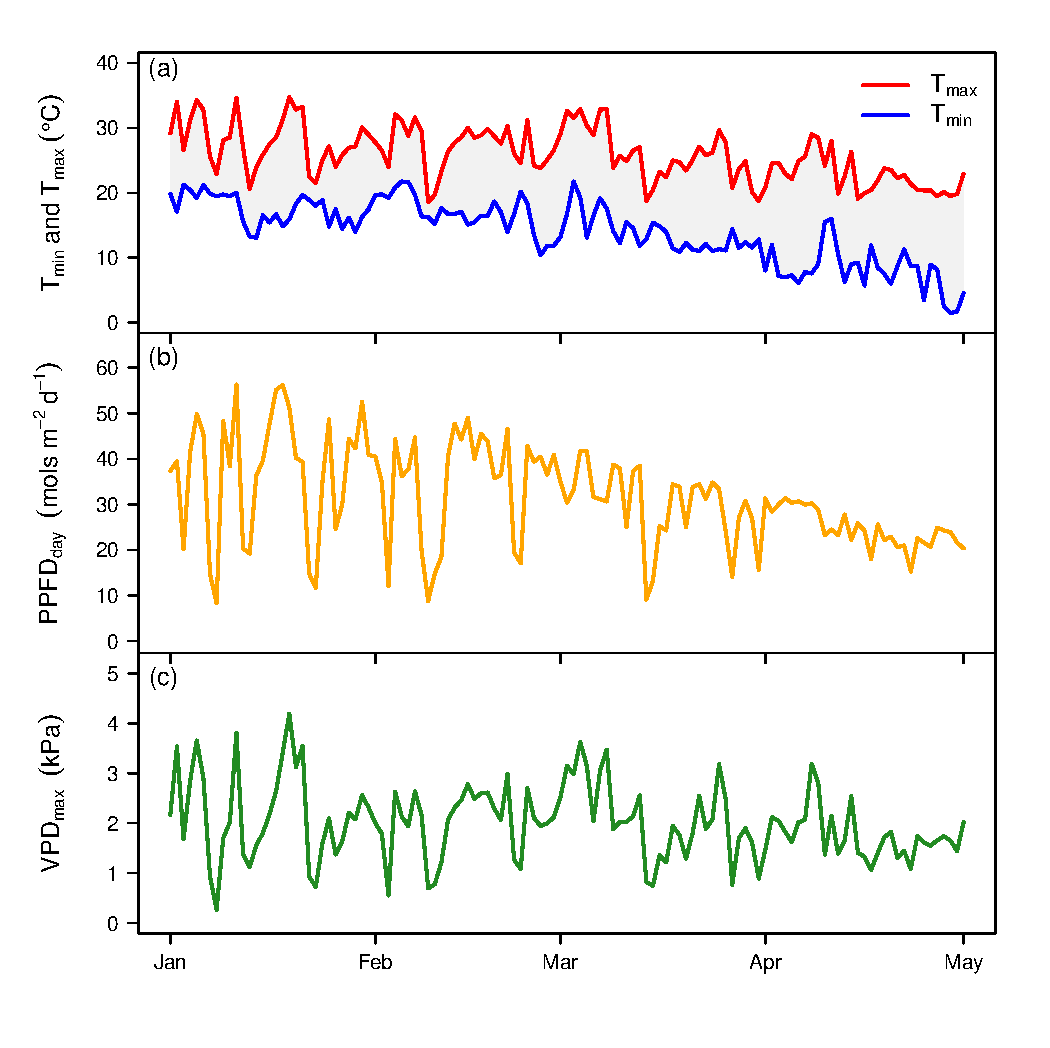
\includegraphics[width=0.99\textwidth]{airvars.pdf}
    \caption{Daily maximum and minimum temperature (a), cumulative daily PPFD (b), and daily maximum vapour pressure deficit (c) across the experiment duration in 2013.}
    \label{fig:figure1}
\end{figure}

%allometry figure
\begin{figure}[h!]
    \centering
    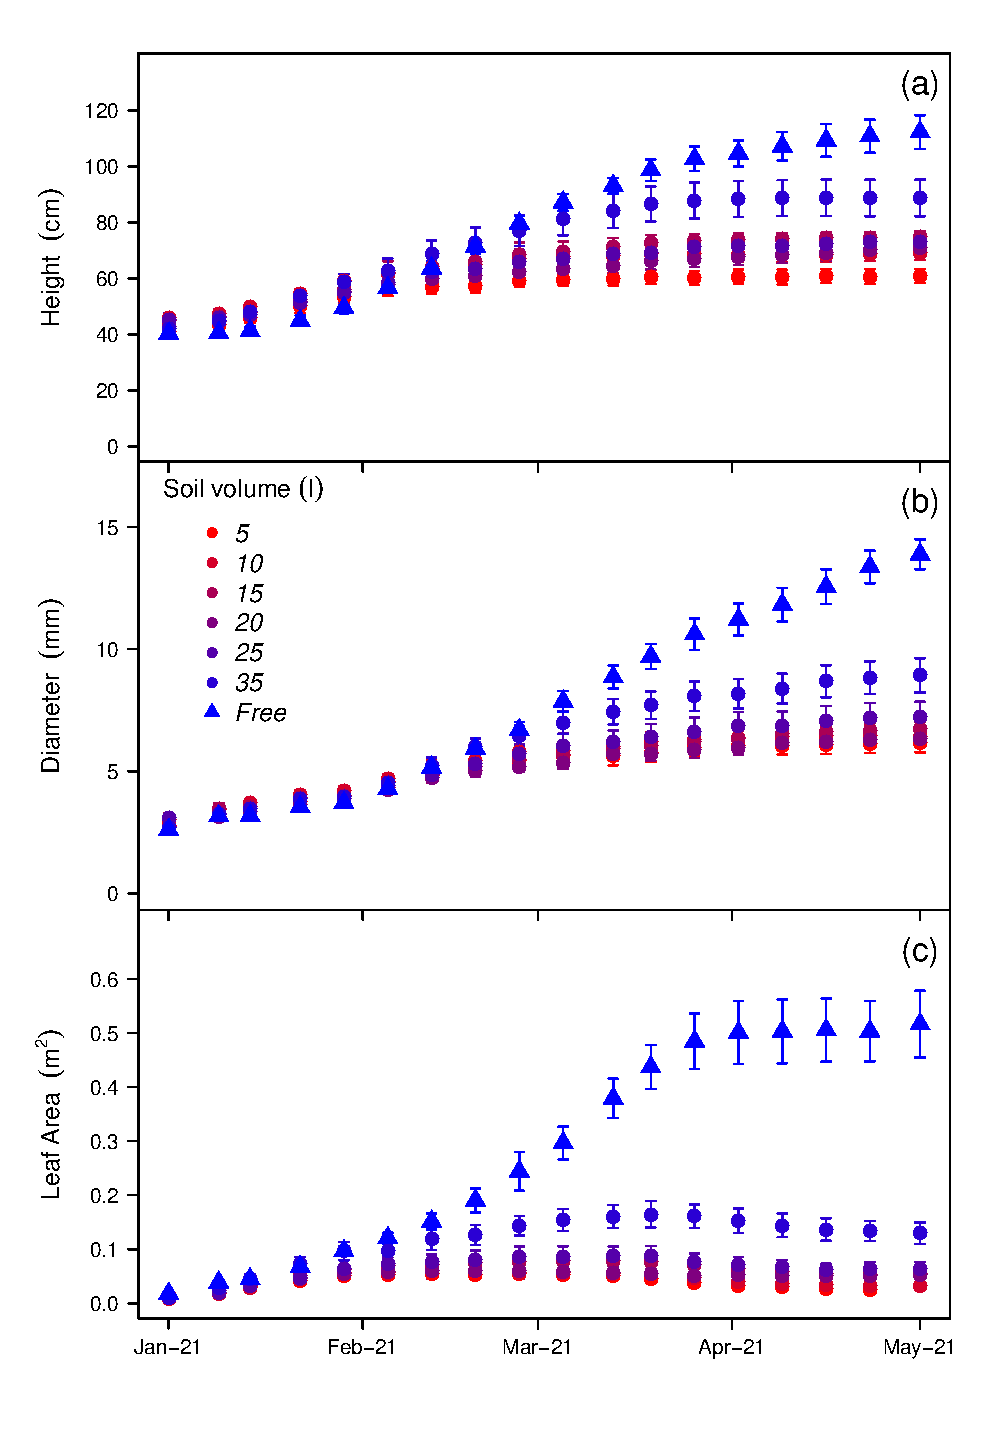
\includegraphics[width=0.99\textwidth]{allometry.pdf}
    \caption{Soil volume treatment means~$\pm$ standard error of height growth (a), diameter growth (b), and interpolated seedling leaf area (c) measured weekly of \textit{Eucalyptus tereticornis} seedlings across the experiment duration in 2013.}
    \label{fig:figure2}
\end{figure}

%asat figure
\begin{figure}[h!]
    \centering
    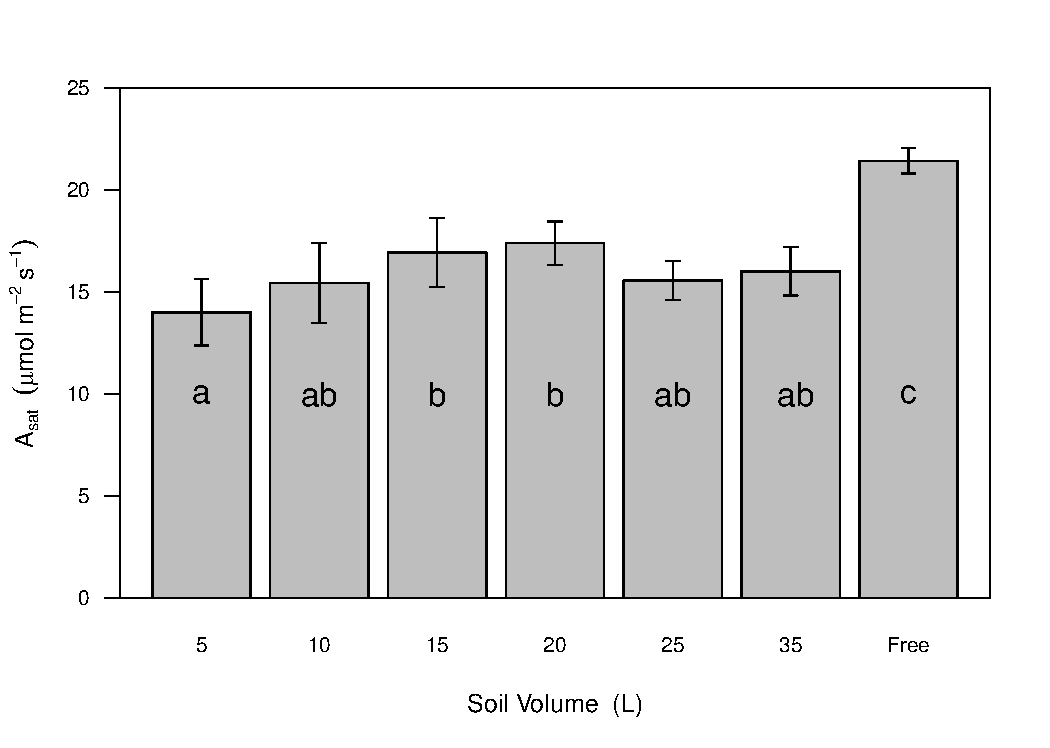
\includegraphics[width=0.99\textwidth]{Asat.pdf}
    \caption{Soil volume treatment means~$\pm$ standard error, across all measurement campaigns (n=6), of light saturated rates of photosynthesis at 25$\degree$C. Different letters represent significant differences between treatments.}
    \label{fig:figure3}
\end{figure}

%partitioning figure
\begin{figure}[h!]
    \centering
    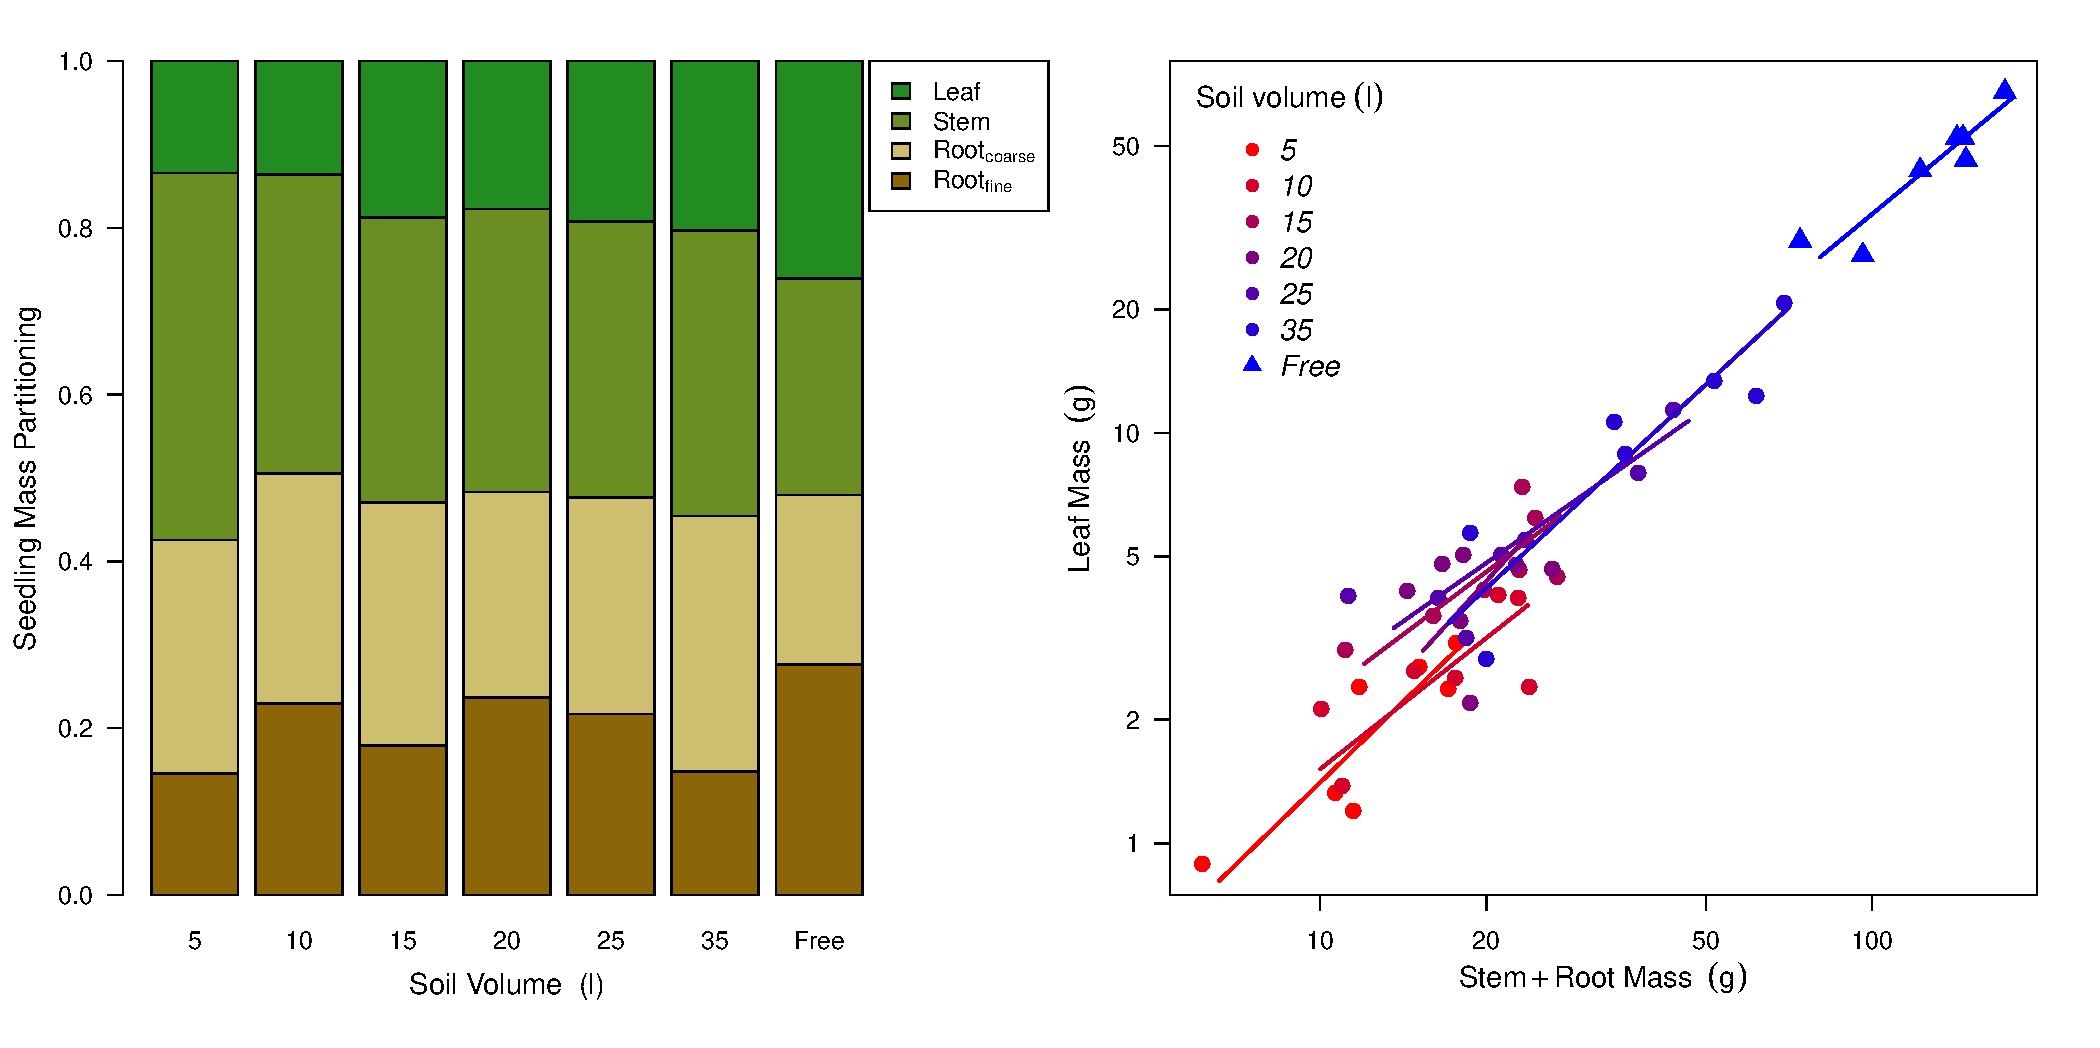
\includegraphics[width=0.99\textwidth]{massfractions.pdf}
    \caption{Soil volume treatment means of mass partitioning to leaves, stems, and roots (a), bi-variate relationships between mass allocation to leaves and stems + roots (b) and leaf mass as a function of fine root biomass $\pm$ standard error (c). For (b) lines represent standardized major axis fitting of the log transformed allometric relationships of leaf mass fraction by treatment.}
    \label{fig:figure4}
\end{figure}

%photochem figure
\begin{figure}[h!]
    \centering
    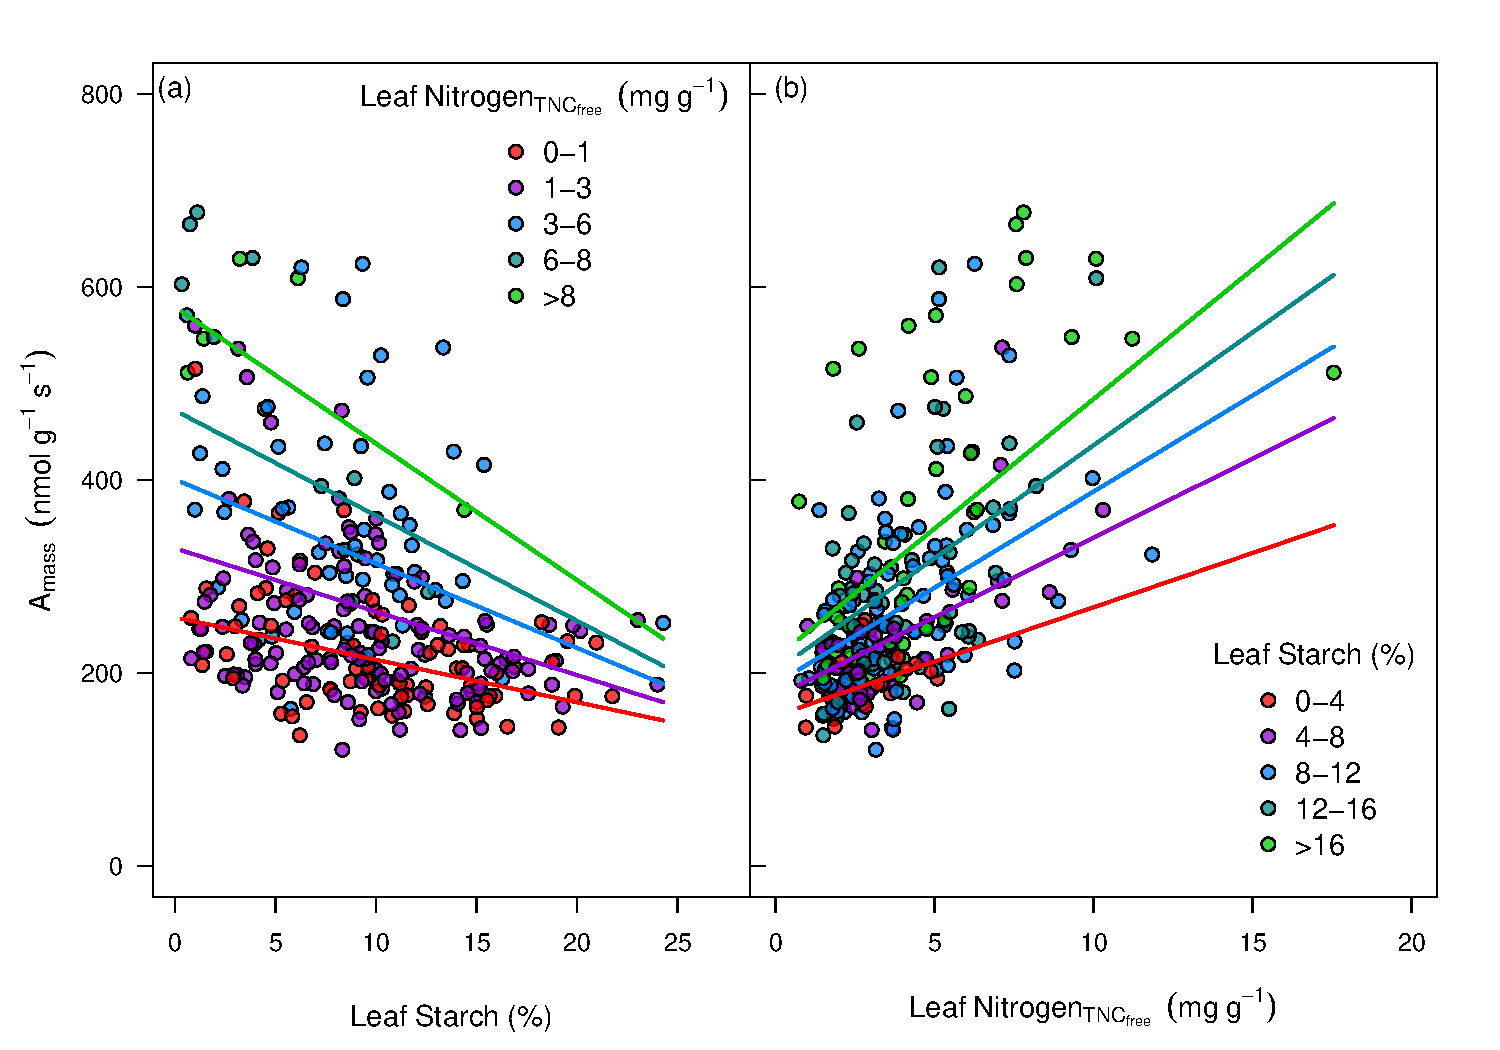
\includegraphics[width=0.99\textwidth]{A_leafchem.pdf}
    \caption{Photosynthetic capacity, on a leaf mass basis, as a function of accumulation of leaf starch (a) and leaf nitrogen content without TNC (b).  Colors represent bins levels (n=5) of both leaf starch and nitrogen grouped from low to high .  Lines represents predictions, for each bin level, from the linear mixed effects model equation of \textit{A}\textsubscript{max} as a function of starch and nitrogen. The marginal \textit{r}\textsuperscript{2} (fixed effects only) was 0.37 and the conditional \textit{r}\textsuperscript{2} (fixed and random effects) was 0.48 for the complete model.}
    \label{fig:figure5}
\end{figure}

%model base figure
\begin{figure}[h!]
    \centering
    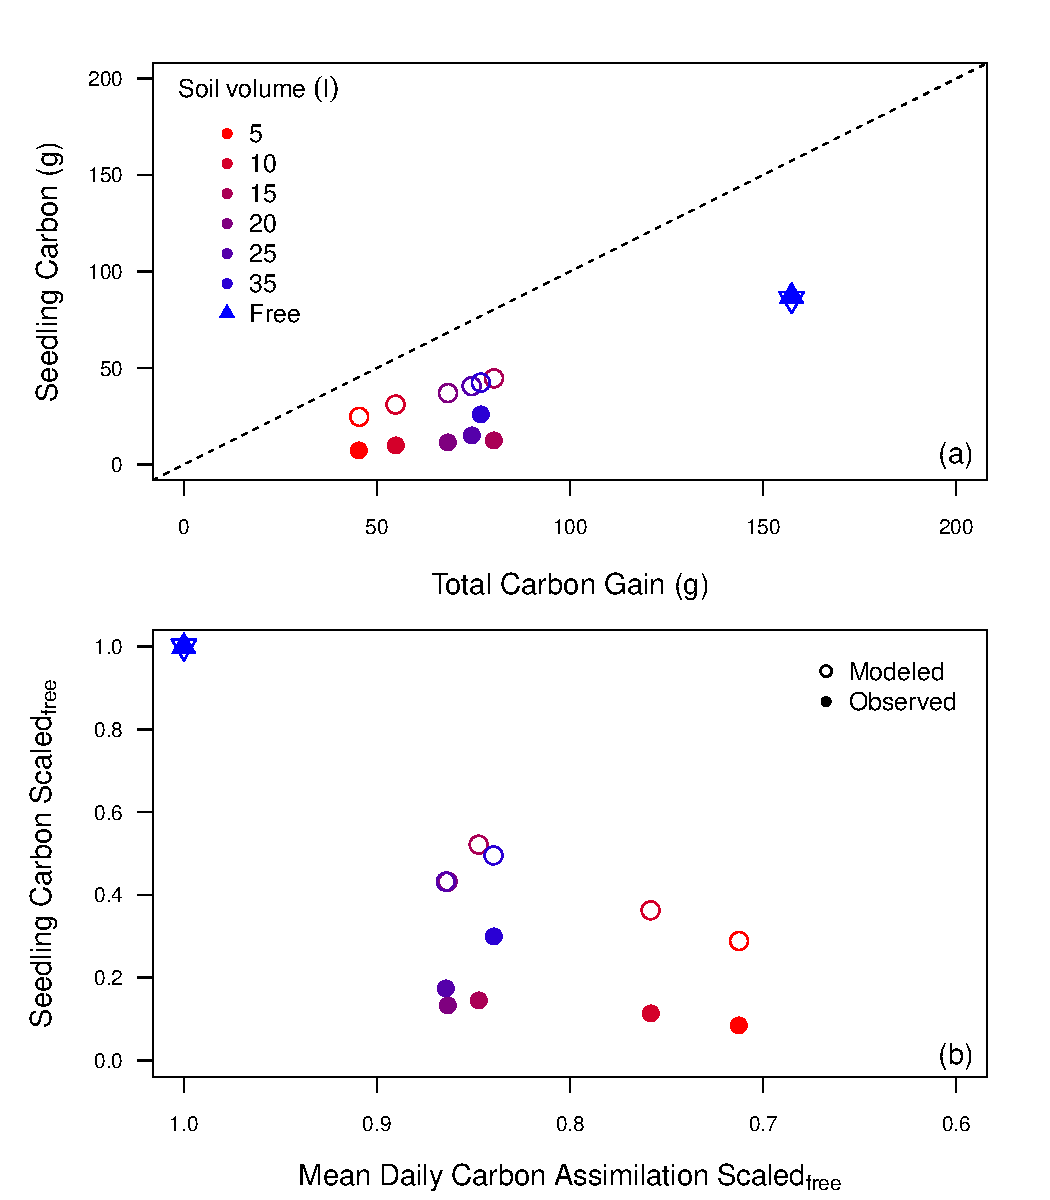
\includegraphics[width=0.99\textwidth]{massmodel_totalC.pdf}
    \caption{Total carbon mass for harvested and modeled seedlings versus predicted total carbon gain after 120 days (a) and  reductions in final seedling carbon mass, both modeled and observed, as a function of the reduction in leaf photosynthesis across treatments (b). For (b) both seedling carbon mass and daily carbon assimilation were first scaled to the free seedling control.}
    \label{fig:figure6}
\end{figure}

%--------------------------------------------------------------------------------------------%
\clearpage
\section{Supporting Information Figures}
% Supporting information. Make sure Figures continue with Fig S1 etc.

\renewcommand\thefigure{S\arabic{figure}}    
\setcounter{figure}{0}   


\begin{figure}[h!]
    \centering
    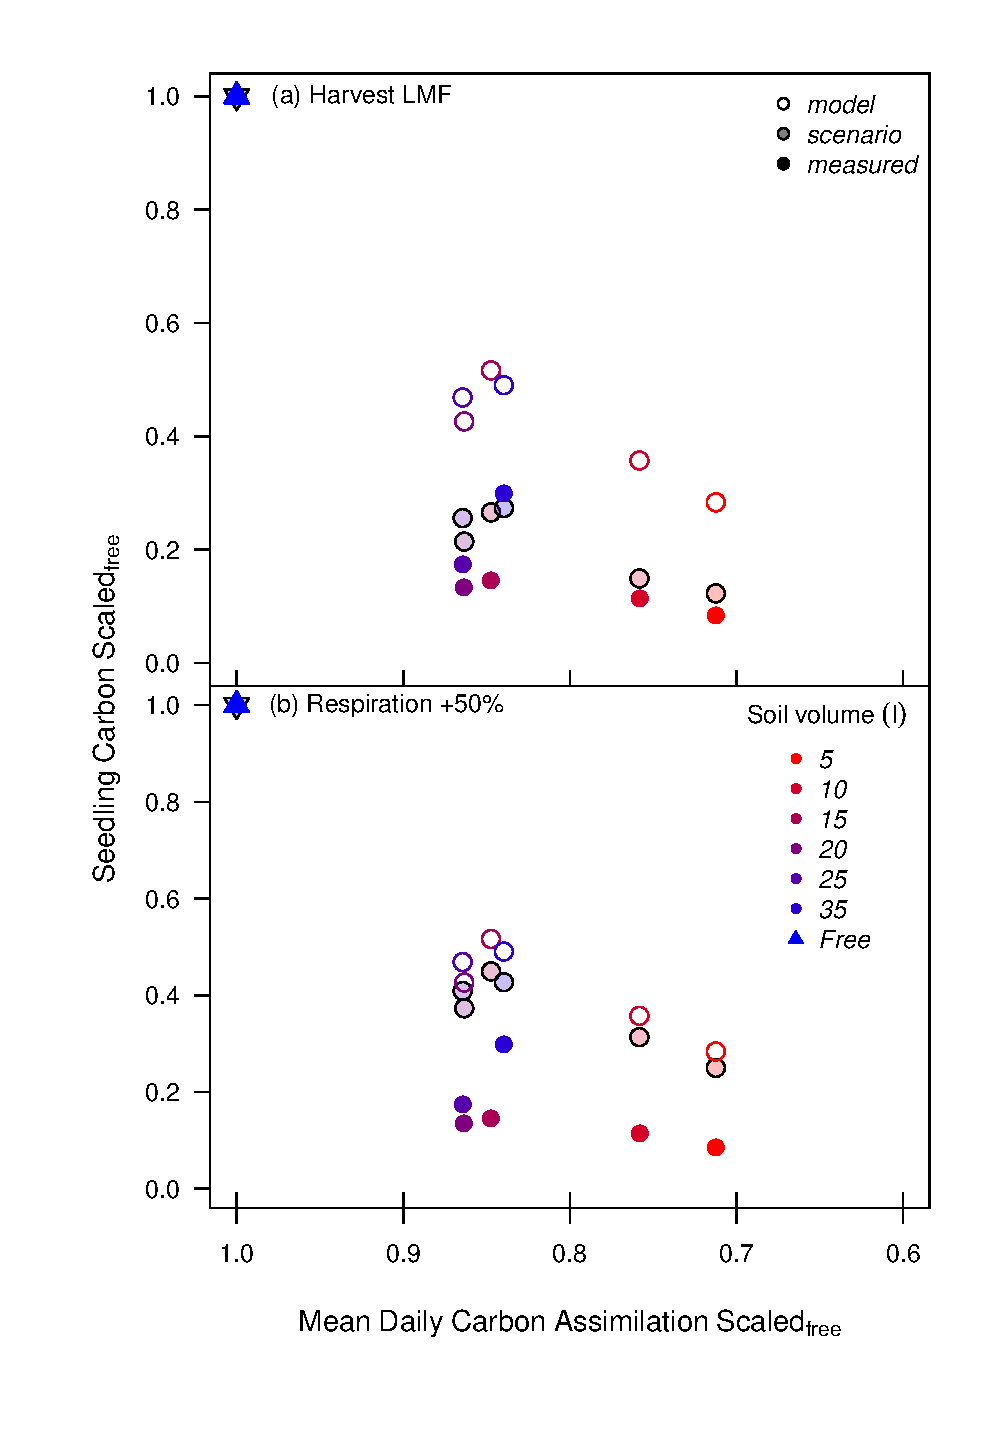
\includegraphics[width=0.99\textwidth]{massmodel_resp.pdf}
    \caption{Sensitivity testing of seedling growth model to different carbon allocation strategies including; constraints of leaf mass fraction to treatment specific final harvest values (a) and changes in respiration of non-leaf tissue components by  $\pm$50~\% (b,c respectively).  Open and filled symbols represent default model and harvest values, while shaded symbols represent model sensitivity to each scenario by soil volume treatment. Both seedling carbon mass and daily carbon assimilation were first scaled to the free seedling control.}
    \label{fig:figureSI1}
\end{figure}


\begin{table}[h!]
  \caption{Seedling Growth Model Default Parameters} 
  \centering 
  \begin{tabular}{l l l l} 
  \hline
  Variable & Default Value & Units & Source  \\ [0.5ex] 
  \hline
  Leaf area\textsubscript{i} & 0.035 & m\textsuperscript{2} & this study \\ 
  Leaf mass\textsubscript{i} & 3.45 & g & this study \\ 
  Stem mass\textsubscript{i} & 1.51 & g & this study \\ 
  Root mass\textsubscript{i} & 0.99 & g & this study \\ 
  \textepsilon\textsubscript{c} & .65 & g~C g~mass\textsuperscript{-1} & \citet{makela1997carbon} \\ 
  R\textsubscript{coarse root} & 0.00124 & g~C g~root\textsuperscript{-1} & \citet{marsden2008relating} \\ 
  R\textsubscript{fine root} & 0.010368 & g~C g~root\textsuperscript{-1} & \citet{ryan2010factors} \\ 
  R\textsubscript{stem} & 0.00187 & g~C g~stem\textsuperscript{-1} & Drake 2014 (unpublished) \\ 
  C\textsubscript{day} & 5.4-7.6 & g~C m\textsuperscript{-2} d\textsuperscript{-1}& this study \\ 
  $\Lambda$ & 1/365 & yr\textsuperscript{-1} & theoretical\\
  \hline 
  \end{tabular}
  \label{table:Table3} 
\end{table}

%--------------------------------------------------------------------------------------------%
\clearpage
\bibliography{pve_cites}

%--------------------------------------------------------------------------------------------%
\end{document}



